\chapter{Desenvolvimento}

Este capítulo apresenta a visão geral do jogo proposto, seus requisitos e principais elementos, como personagens e ambientes. Também são detalhados os objetivos e mecânicas do jogo e suas cenas.

\section{Visão Geral}

O jogo é chamado ``Mistério Financeiro: A Jornada de Chico''. No início o protagonista Chico se depara com o mistério das despesas crescentes e do desaparecimento de moedas na papelaria de sua família. Motivado por um senso de responsabilidade, ele decide investigar o caso. A investigação começa pelo porão da loja, um local pouco visitado pela sua família.

A narrativa avança através de uma série de desafios e escolhas que Chico deve enfrentar. Essas decisões vão desde escolhas cotidianas, como a compra de um relógio, até interações complexas com personagens, como seu amigo Vicente. Cada escolha tem um impacto na história e nas lições de economia e gestão financeira apresentadas.

À medida que Chico investiga, ele descobre várias causas para os problemas financeiros da papelaria, desde descuidos simples até ações mal-intencionadas de terceiros. O jogo ressalta a importância da atenção aos detalhes e do controle de gastos para a saúde financeira de um negócio.

O jogo é estruturado de forma interativa, oferecendo múltiplos finais baseados nas decisões do jogador ao longo de sua experiência. Isso enfatiza a relevância de escolhas responsáveis e informadas, tanto no jogo quanto na vida real. Neste sentido, o jogo incorpora um forte elemento educacional, enfatizando conceitos de gestão financeira. Ele ensina sobre a importância do planejamento financeiro, economia e investimentos, incentivando os jogadores a refletirem sobre suas próprias decisões financeiras.

\section{Requisitos de Software}

\subsection*{Requisitos Funcionais}
\begin{itemize}
	\item RF1. O jogo deve oferecer uma interface gráfica interativa, simbolizando os diferentes ambientes da história de Chico.
	\item RF2. Incluir um sistema de diálogo interativo com personagens, como Seu Mário, Vicente, Luiza, entre outros.
	\item RF3. Permitir que o jogador faça escolhas que influenciam o desenvolvimento da história e interações com personagens.
	\item RF4. Permitir a compra e uso de itens para progredir na narrativa, principalmente se tratando da lanterna que será usada para verificar o porão.
	\item RF5. Apresentar múltiplos finais com base nas decisões tomadas pelo jogador, influenciadas pelas interações com personagens.
	\item RF6. Incorporar elementos de educação financeira dentro da narrativa e desafios, utilizando situações da história de Chico como exemplos.
\end{itemize}

\subsection*{Requisitos Não Funcionais}
\begin{itemize}
	\item RNF1. O jogo deve ter uma interface gráfica atrativa e intuitiva, adequada para a faixa etária do 5º ano do Ensino Fundamental.
	\item RNF2. O jogo deve ser otimizado para um desempenho fluido, sem atrasos ou erros técnicos.
	\item RNF3. O jogo deve ser compatível com a plataforma Windows, MacOS e Web.
	\item RNF4. O jogo deve ter uma trilha sonora e efeitos sonoros imersivos, complementando a experiência visual.
\end{itemize}

\subsection*{Regras de Negócio}
\begin{itemize}
	\item RN1. A história deve se adaptar e mudar com base nas escolhas feitas pelo jogador (RF3, RF5).
	\item RN2. Os desafios e enigmas devem ser integrados na história e contribuir para o aprendizado sobre finanças (RF4, RF6).
	\item RN3. Os diálogos e interações com personagens devem oferecer pistas e informações relevantes para a progressão da história (RF2).
	\item RN4. O jogo deve promover a conscientização sobre gestão financeira e economia de forma lúdica e educativa (RF6).\com{Pode incluir uma última RN de que os elementos e enredo do jogo devem seguir a história x do livro y da ENEF.}
\end{itemize}

\section{Elementos do Jogo}

\subsection{Personagens e Ambientes}
Esta seção detalha os personagens não jogáveis (NPCs, do inglês \textit{non-player character}) e os ambientes (também chamados de \textit{mapas}) que serão fundamentais para a narrativa e jogabilidade do jogo. Cada NPC e mapa pode ser acompanhado de uma imagem e uma descrição detalhada para melhor imersão e compreensão do jogador.

\icom{Colocar todas as imagens dos NPCs em uma figura única, cuja legenda será ``Imagens de cada NPC.''. Abaixo de cada imagem, colocar o nome do NPC (por exemplo, Seu Mário).}

O jogo apresenta os NPCs apresentados na Figura~\ref{fig:npcs}. Abaixo, é fornecida uma descrição para cada um deles.

\icom{É bom evitar o abuso de itemize. Uma forma de apresentação alternativa é apresentada abaixo.}

\medskip\noindent \textbf{Seu Mário.}\quad Pai de Chico, dedicado dono da papelaria da família. Enfrenta desafios financeiros e tenta manter o negócio próspero.

\medskip\noindent \textbf{Pai do Vicente.}\quad Aparece na história para repreender seu filho por envolvimento em furtos, refletindo preocupação paterna diante da situação indesejada.

\medskip\noindent \textbf{Atendente da Loja de Itens.}\quad Caracterizado como um comerciante prestativo, interage com Chico durante a compra do seu relógio.

\medskip\noindent \textbf{Vicente.}\quad Colega de escola de Chico, conhecido por seu comportamento provocativo e envolvimento em pequenos furtos.

\medskip\noindent \textbf{Luiza.}\quad Melhor amiga de Chico, sempre oferecendo apoio e aconselhamento nas aventuras e desafios enfrentados por ele.

\medskip\noindent \textbf{Maria José.}\quad Mãe de Chico, auxilia na papelaria e compartilha das preocupações financeiras da família.

\medskip\noindent \textbf{Josimar.}\quad Funcionário da papelaria, inicialmente suspeito de furto, revelando-se inocente e um aliado importante.

\medskip\noindent \textbf{Ratazana.}\quad Uma ameaça inesperada no porão da papelaria, adicionando suspense e desafios físicos à narrativa.

\medskip\noindent \textbf{Atendente do Hospital.}\quad Representa um ponto de contato no cenário hospitalar, caso Chico necessite de cuidados médicos devido ao ataque da ratazana.

\medskip\noindent \textbf{Médico.}\quad Figura de cuidado e autoridade, que atende Chico no hospital após eventuais incidentes.

\medskip\noindent \textbf{Atendente da Loja de Ferragens.}\quad Ajuda Chico na aquisição da lanterna, útil durante suas investigações.

\medskip\noindent \textbf{Cida.}\quad Irmã mais nova de Chico, envolvida nos dilemas familiares e curiosa sobre os mistérios da papelaria.

\medskip\noindent \textbf{Personagens não nomeados (4).}\quad Personagens secundários, aparecem apenas para compor algumas cenas, como o encontro com os amigos da escola na lanchonete.

%\begin{figure}[ht]
%	\centering
%	\caption{NPC Seu Mário.}
%	
\includegraphics[scale=0.8]{Textuais/Pictures/Seu_Mario.png}
%	\fonte{Criado pelo Autor.}\label{fig:npc-seu-mario}
%\end{figure}
%
%\begin{figure}[ht]
%	\centering
%	\caption{NPC Pai do Vicente.}
%	
\includegraphics[scale=0.8]{Textuais/Pictures/Pai_Vicente.png}
%	\fonte{Criado pelo Autor.}\label{fig:npc-pai-vicente}
%\end{figure}
%
%\begin{figure}[ht]
%	\centering
%	\caption{NPC Atendente da Loja de Itens.}
%	
\includegraphics[scale=0.8]{Textuais/Pictures/Atendente_loja_Itens.png}
%	\fonte{Criado pelo Autor.}\label{fig:npc-atendente-loja-itens}
%\end{figure}
%
%\begin{figure}[ht]
%	\centering
%	\caption{NPC Vicente.}
%	
\includegraphics[scale=0.8]{Textuais/Pictures/Vicente.png}
%	\fonte{Criado pelo Autor.}\label{fig:npc-vicente}
%\end{figure}
%
%\begin{figure}[ht]
%	\centering
%	\caption{NPC Luiza.}
%	\includegraphics[scale=0.8]{Textuais/Pictures/Luísa.png}
%	\fonte{Criado pelo Autor.}\label{fig:npc-luiza}
%\end{figure}
%
%\begin{figure}[ht]
%	\centering
%	\caption{NPC Maria José.}
%	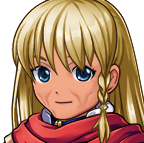
\includegraphics[scale=0.8]{Textuais/Pictures/Maria.png}
%	\fonte{Criado pelo Autor.}\label{fig:npc-maria-jose}
%\end{figure}
%
%\begin{figure}[ht]
%	\centering
%	\caption{NPC Josimar.}
%	
\includegraphics[scale=0.8]{Textuais/Pictures/Josimar.png}
%	\fonte{Criado pelo Autor.}\label{fig:npc-josimar}
%\end{figure}
%
%\begin{figure}[ht]
%	\centering
%	\caption{NPC Ratazana.}
%	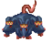
\includegraphics[scale=1.8]{Textuais/Pictures/Ratazana.png}
%	\fonte{Hellpug/Emily Lampson.}\label{fig:npc-ratazana}
%\end{figure}
%
%\begin{figure}[ht]
%	\centering
%	\caption{NPC Atendente do Hospital.}
%	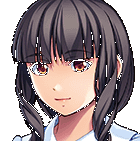
\includegraphics[scale=0.8]{Textuais/Pictures/Atendente_Hospital.png}
%	\fonte{\textit{Asset} padrão do RPG Maker MZ.}\label{fig:npc-atendente-hospital}
%\end{figure}
%
%\begin{figure}[ht]
%	\centering
%	\caption{NPC Médico.}
%	
\includegraphics[scale=0.8]{Textuais/Pictures/Medico.png}
%	\fonte{\textit{Asset} padrão do RPG Maker MZ.}\label{fig:npc-medico}
%\end{figure}
%
%\begin{figure}[ht]
%	\centering
%	\caption{NPC Atendente da Loja de Ferragens.}
%	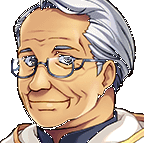
\includegraphics[scale=0.8]{Textuais/Pictures/Atendente_Loja_Ferragens.png}
%	\fonte{\textit{Asset} padrão do RPG Maker MZ.}\label{fig:npc-atendente-loja-ferragens}
%\end{figure}
%
%\begin{figure}[ht]
%	\centering
%	\caption{NPC Cida.}
%	
\includegraphics[scale=0.8]{Textuais/Pictures/Cida.png}
%	\fonte{Criado pelo autor.}\label{fig:npc-cida}
%\end{figure}

\bigskip\medskip
O jogo ainda apresenta nove ambientes, os quais estão apresentados nas Figuras~\ref{fig:mundo-chico}~--~\ref{fig:casa-chico}. Os detalhes de cada ambiente são fornecidos abaixo.

\icom{Fazer a listagem e descrições de cada cenário conforme feito com os NPCs. Deixar as figuras depois do texto. Após detalhar o ambiente, referenciar a figura correspondente, conforme feito no ``Mundo de Chico''.}

\medskip\noindent \textbf{Mundo do Chico.}\quad O cenário geral da aventura, que inclui a vizinhança, ruas e locais frequentados por Chico e seus amigos (Figura~\ref{fig:mundo-chico}).

\begin{itemize}
	      \begin{figure}[ht]
		      \centering
		      \caption{Mapa Mundo Chico.}
		      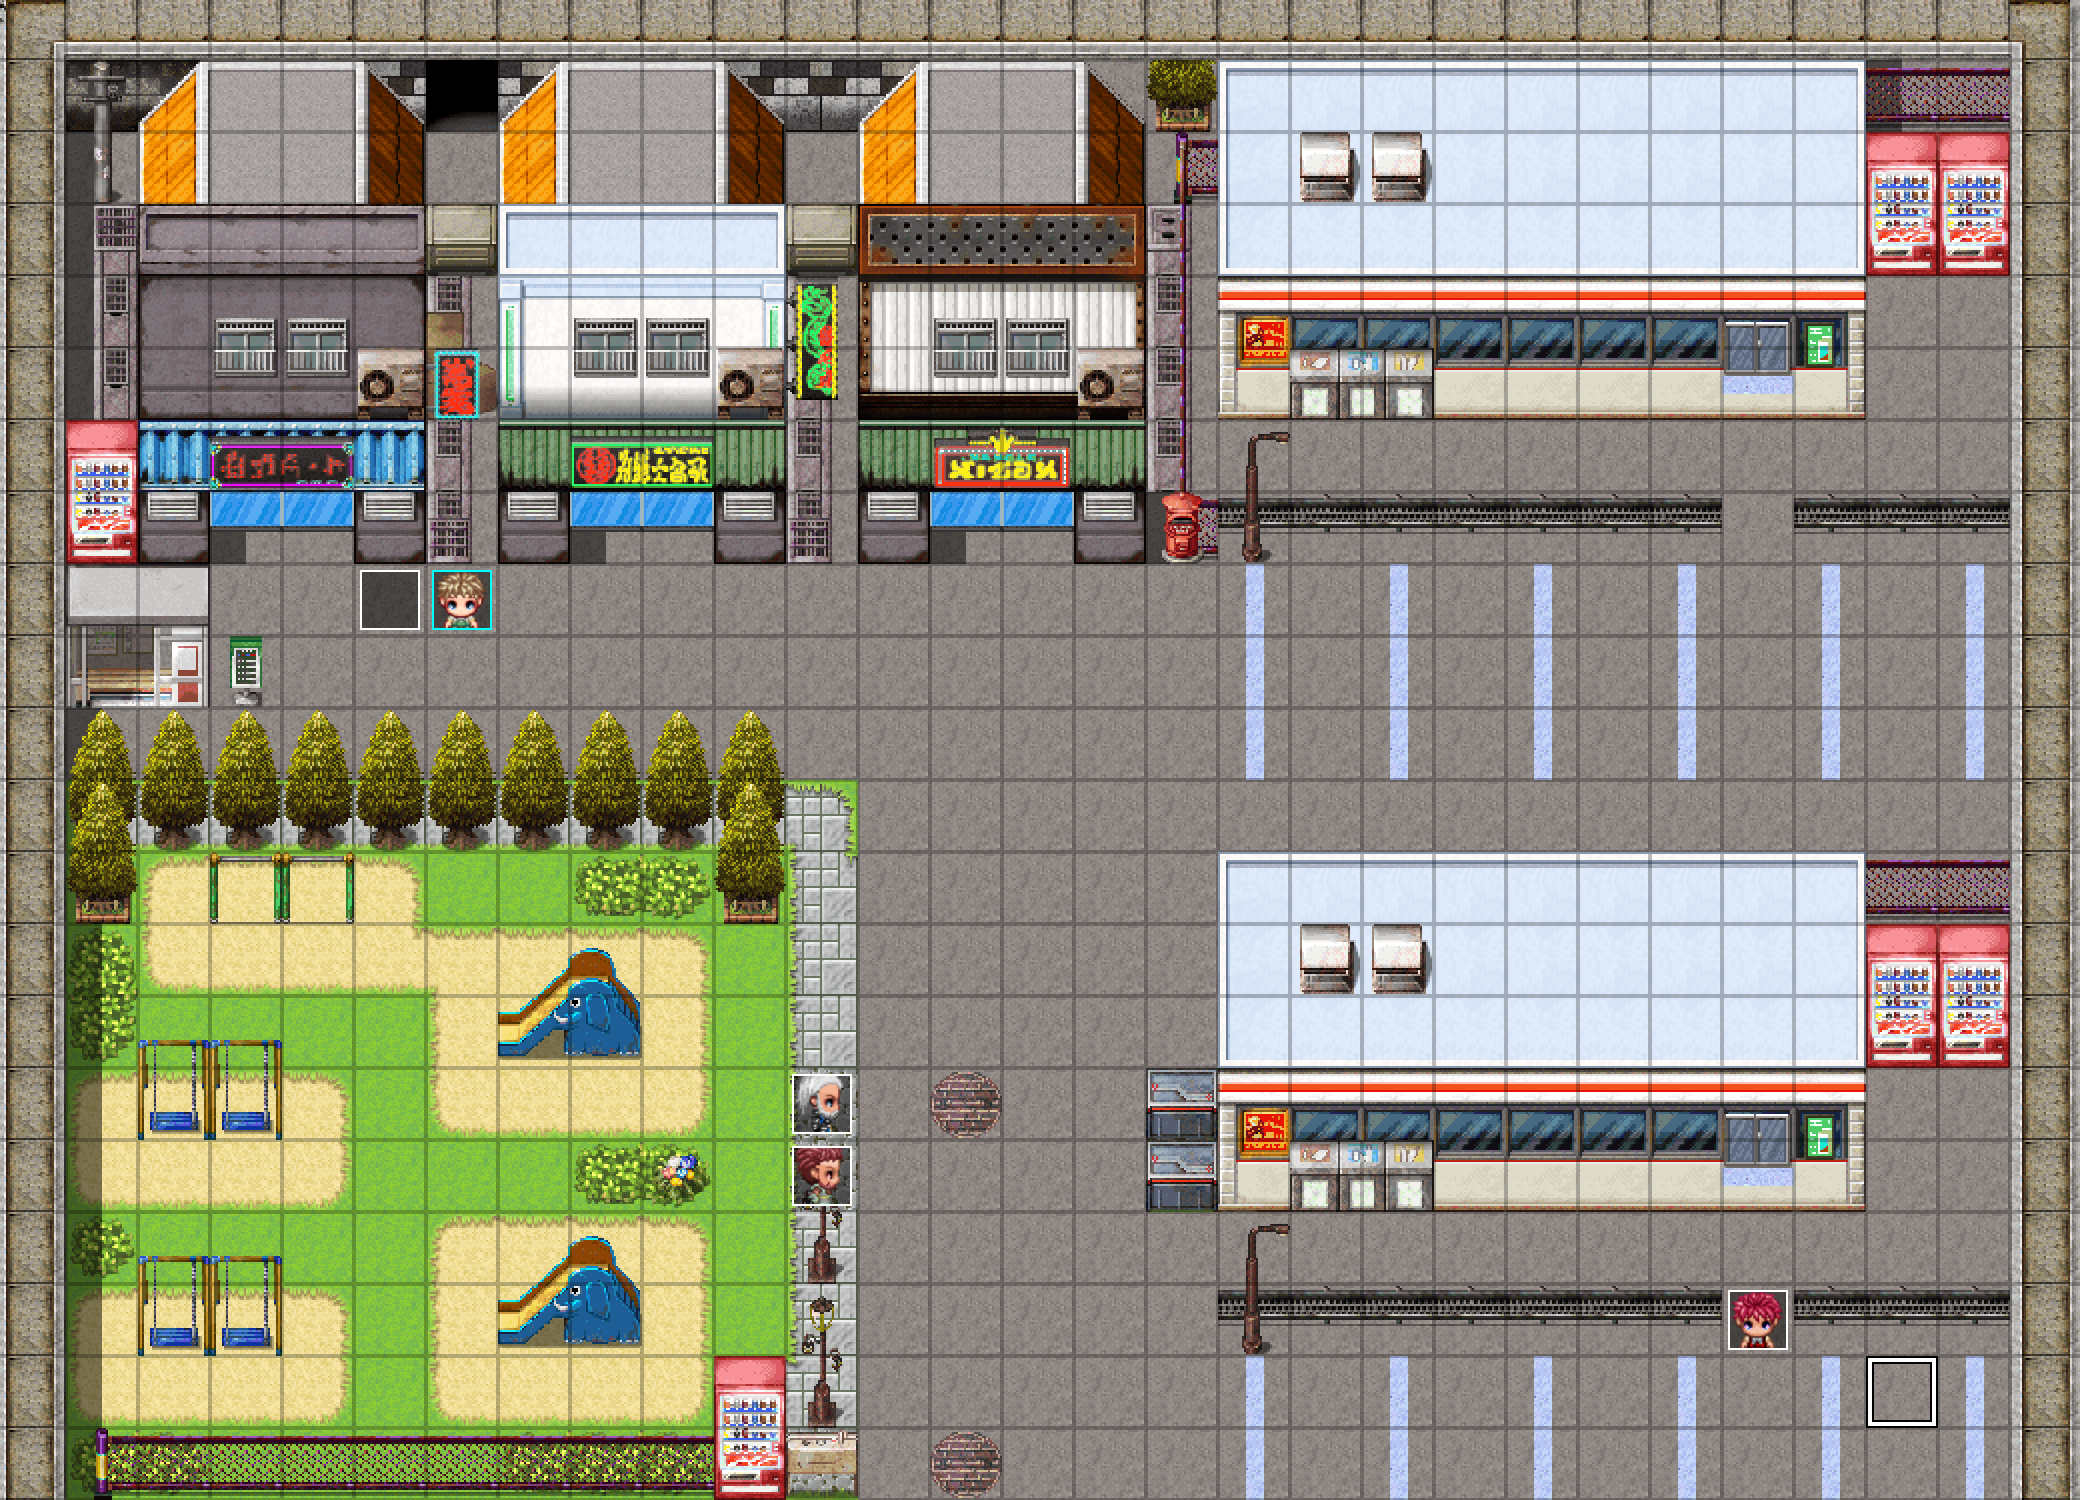
\includegraphics[scale=0.3]{Textuais/Pictures/Mundo_chico.png}
		      \fonte{Criado pelo autor.}\label{fig:mundo-chico}
	      \end{figure}


	\item Loja de Itens: Estabelecimento onde Chico adquire itens como o relógio.

	      \begin{figure}[ht]
		      \centering
		      \caption{Mapa Loja de Itens.}
		      \includegraphics[scale=0.4]{Textuais/Pictures/Loja_itens.png}
		      \fonte{Criado pelo autor.}\label{fig:loja-itens}
	      \end{figure}

	      \newpage

	\item Lanchonete: Espaço social para Chico e seus amigos, propício para conversas e desenvolvimento de subtramas.

	      \begin{figure}[ht]
		      \centering
		      \caption{Mapa Lanchonete.}
		      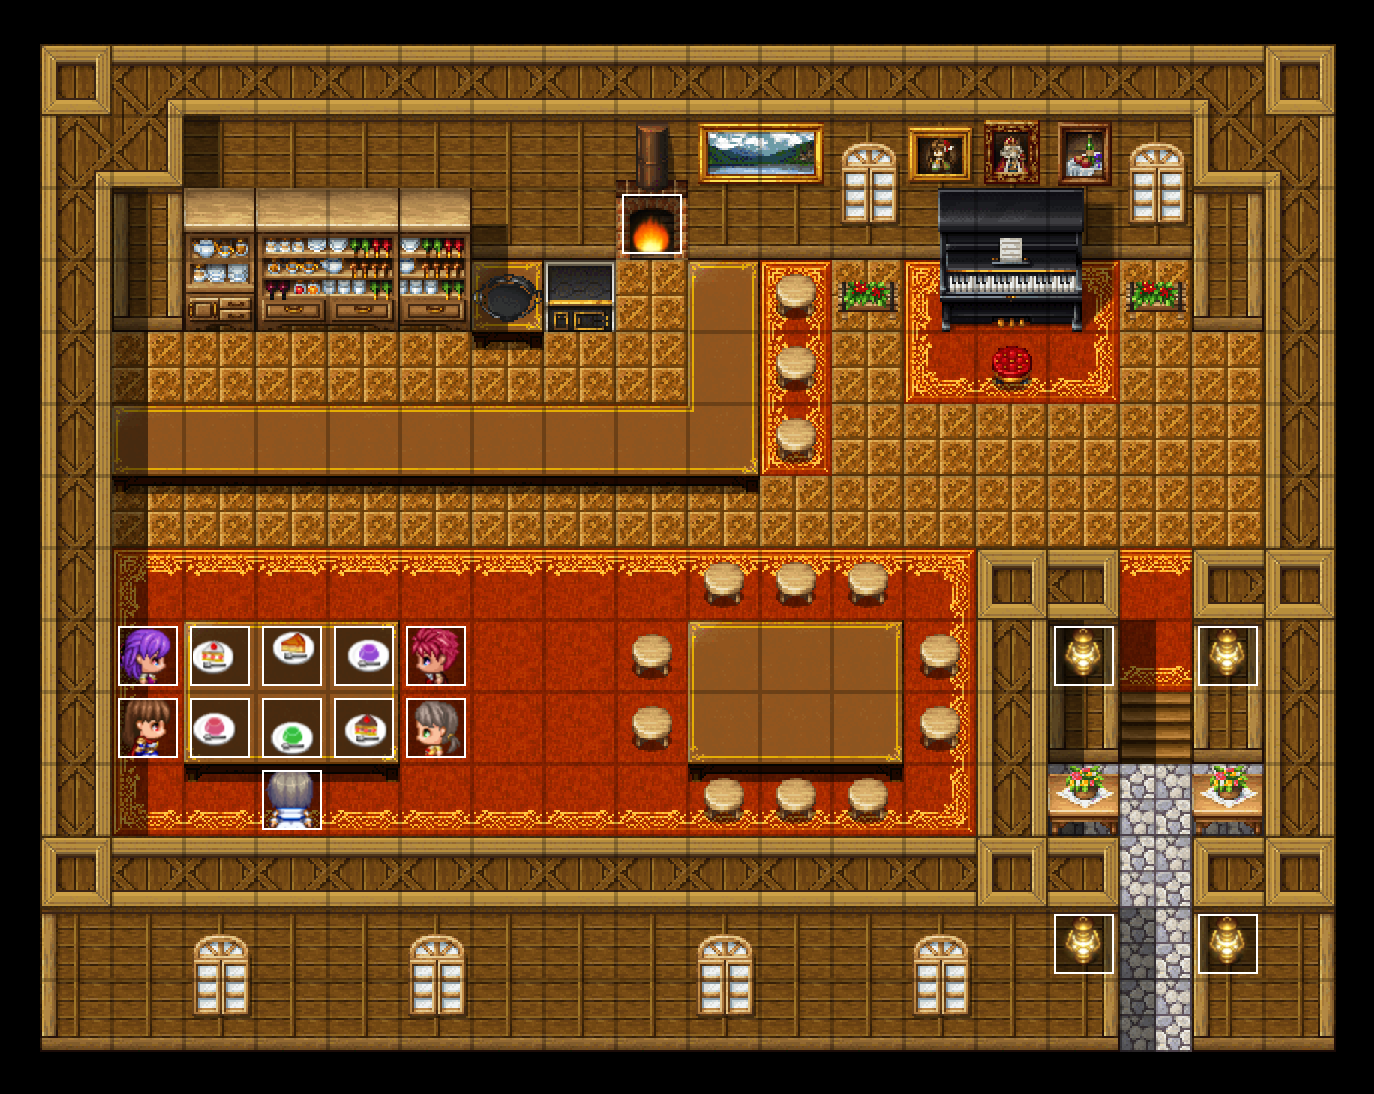
\includegraphics[scale=0.4]{Textuais/Pictures/Lanchonete.png}
		      \fonte{Criado pelo autor.}\label{fig:lanchonete}
	      \end{figure}

	\item Papelaria da Família: Coração da trama, onde muitos dos mistérios e desafios se concentram.

	      \begin{figure}[ht]
		      \centering
		      \caption{Mapa Papelaria.}
		      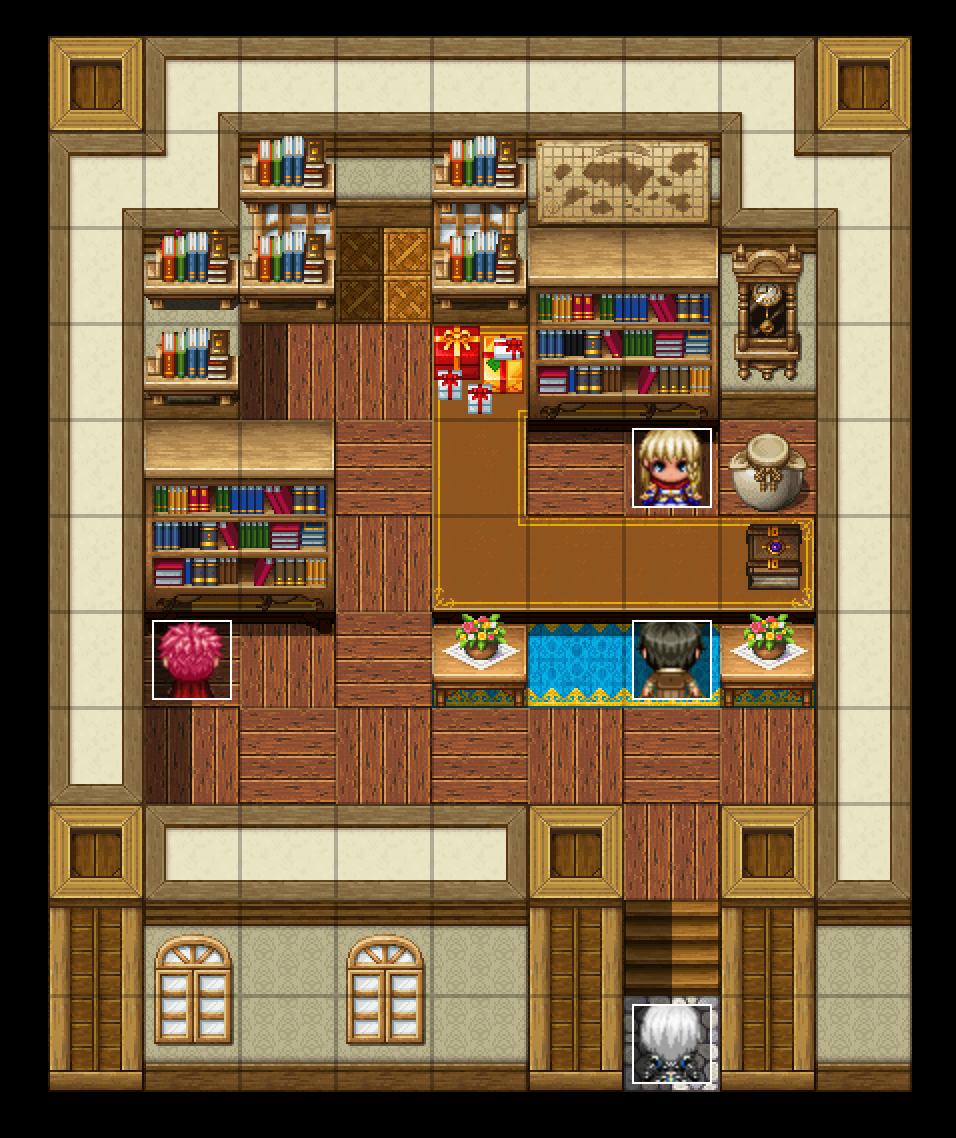
\includegraphics[scale=0.5]{Textuais/Pictures/Papelaria_Familia.png}
		      \fonte{Criado pelo autor.}\label{fig:papelaria-familia}
	      \end{figure}

	\item Cozinha da Papelaria: Local onde Chico encontra o Josimar e faz descobertas, como o problema com a geladeira.

	      \begin{figure}[ht]
		      \centering
		      \caption{Mapa da cozinha da papelaria.}
		      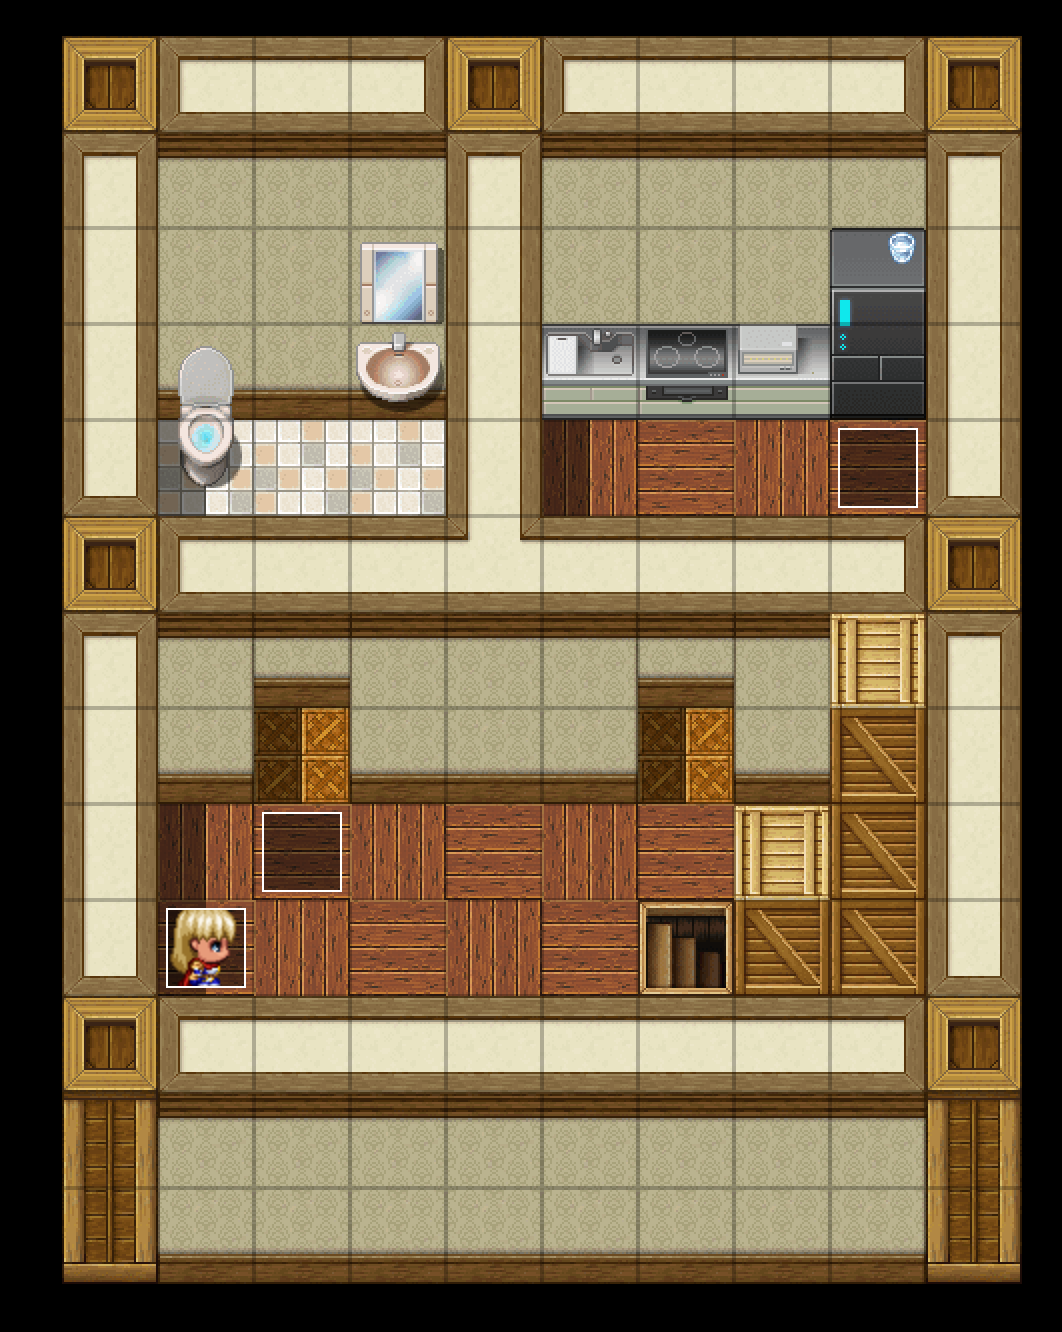
\includegraphics[scale=0.5]{Textuais/Pictures/Cozinha_papelaria.png}
		      \fonte{Criado pelo autor.}\label{fig:lanchonete}
	      \end{figure}

	\item Porão da Papelaria: Ambiente sombrio e cheio de mistérios, onde Chico enfrenta a Ratazana.

	      \begin{figure}[ht]
		      \centering
		      \caption{Mapa do porão da papelaria.}
		      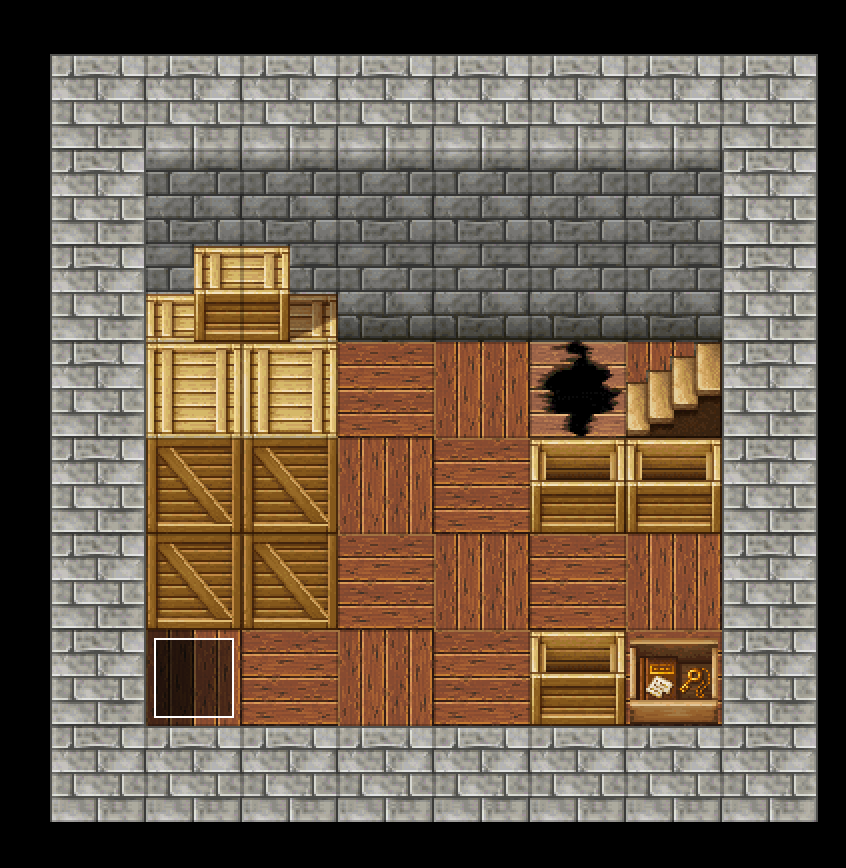
\includegraphics[scale=0.4]{Textuais/Pictures/Porao_papelaria.png}
		      \fonte{Criado pelo autor.}\label{fig:porao-papelaria}
	      \end{figure}

	\item Hospital: Local de cuidado e recuperação, podendo ser cenário de eventos dramáticos, como o ataque da ratazana.

	      \begin{figure}[ht]
		      \centering
		      \caption{Mapa do hospital.}
		      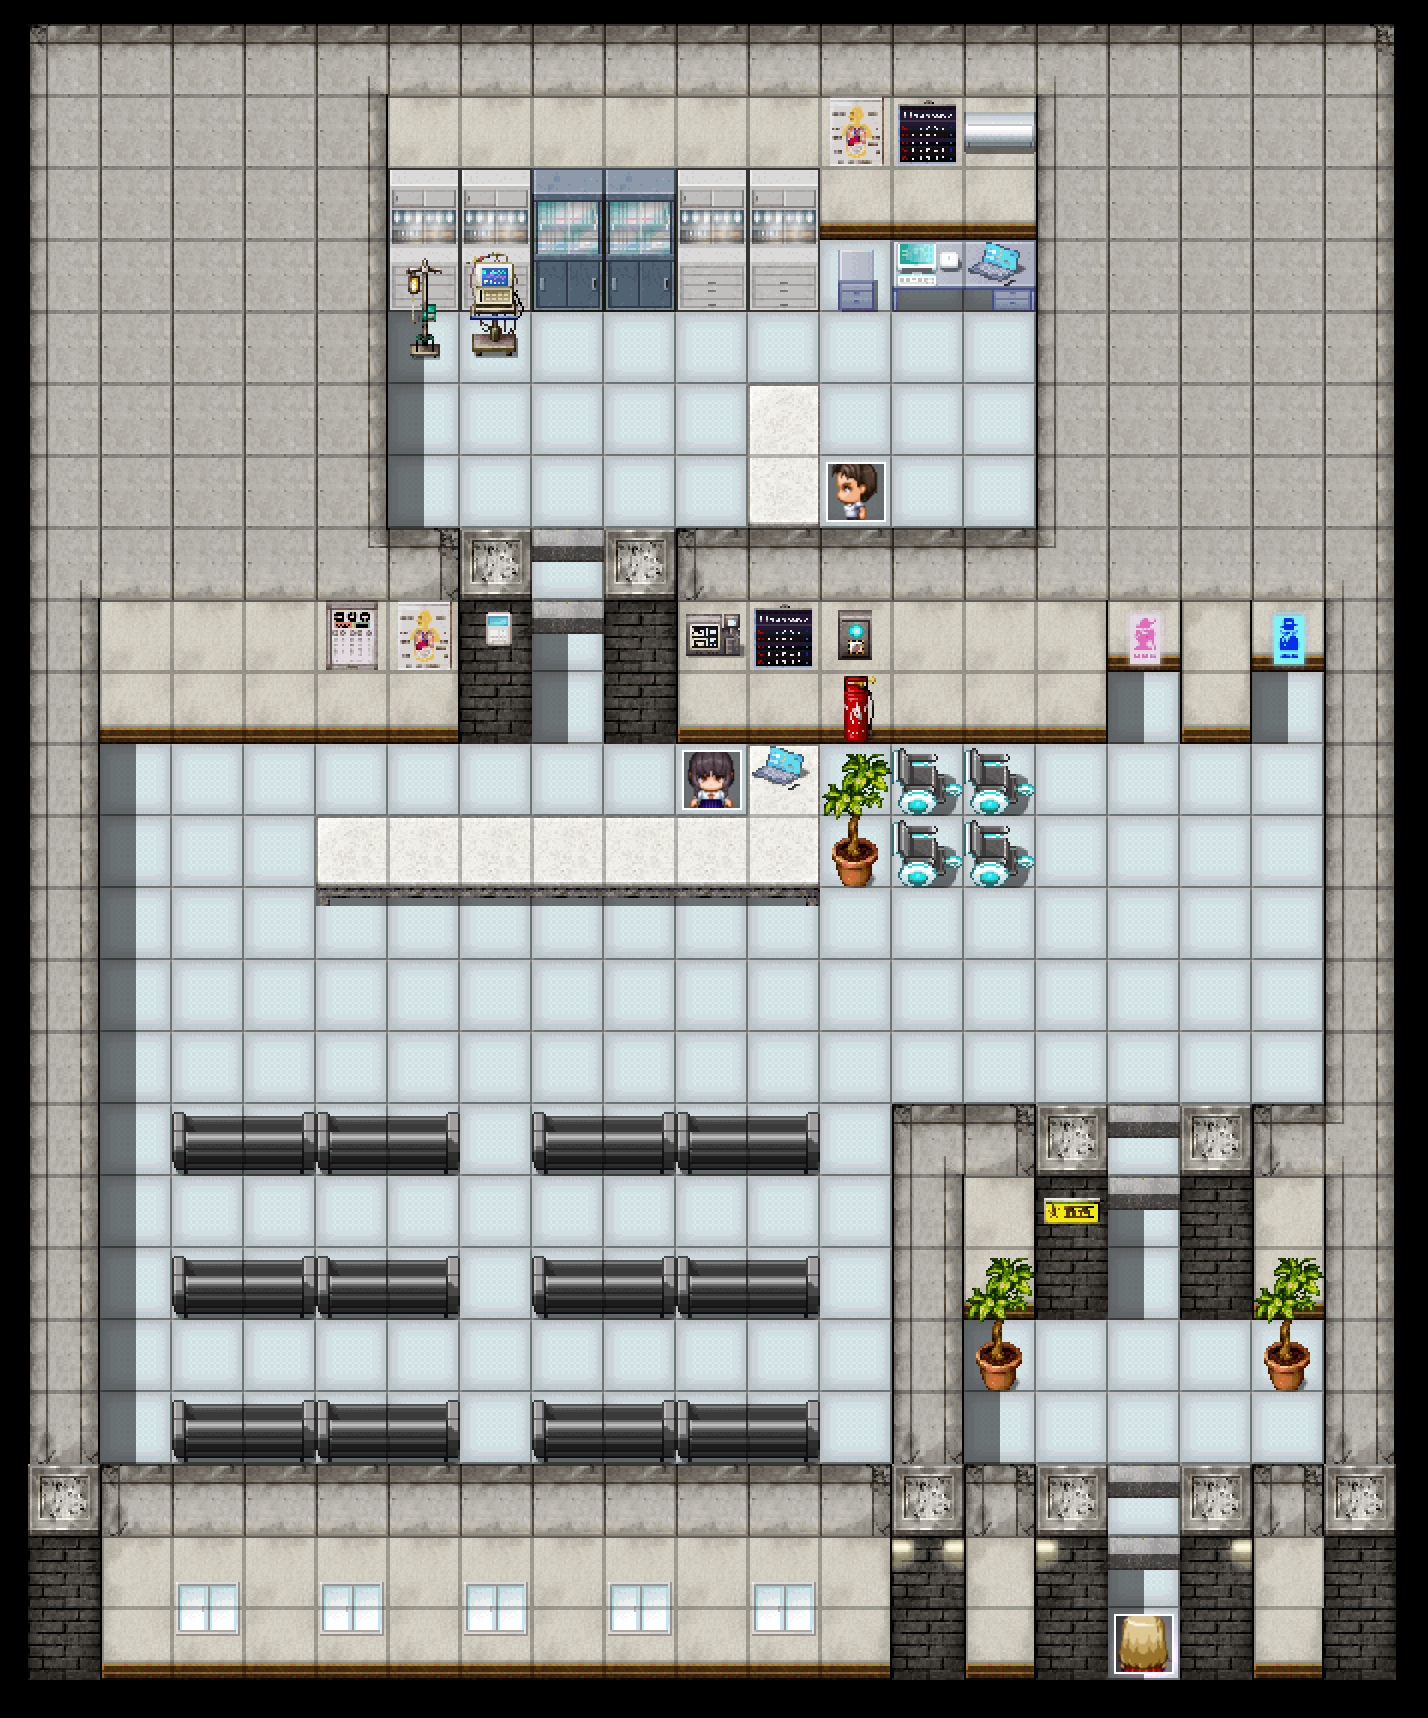
\includegraphics[scale=0.5]{Textuais/Pictures/Hospital.png}
		      \fonte{Criado pelo autor.}\label{fig:hospital}
	      \end{figure}

	      \newpage

	\item Loja de Ferragens: Fornecedora da lanterna para as investigações de Chico.

	      \begin{figure}[ht]
		      \centering
		      \caption{Mapa da loja de ferragens.}
		      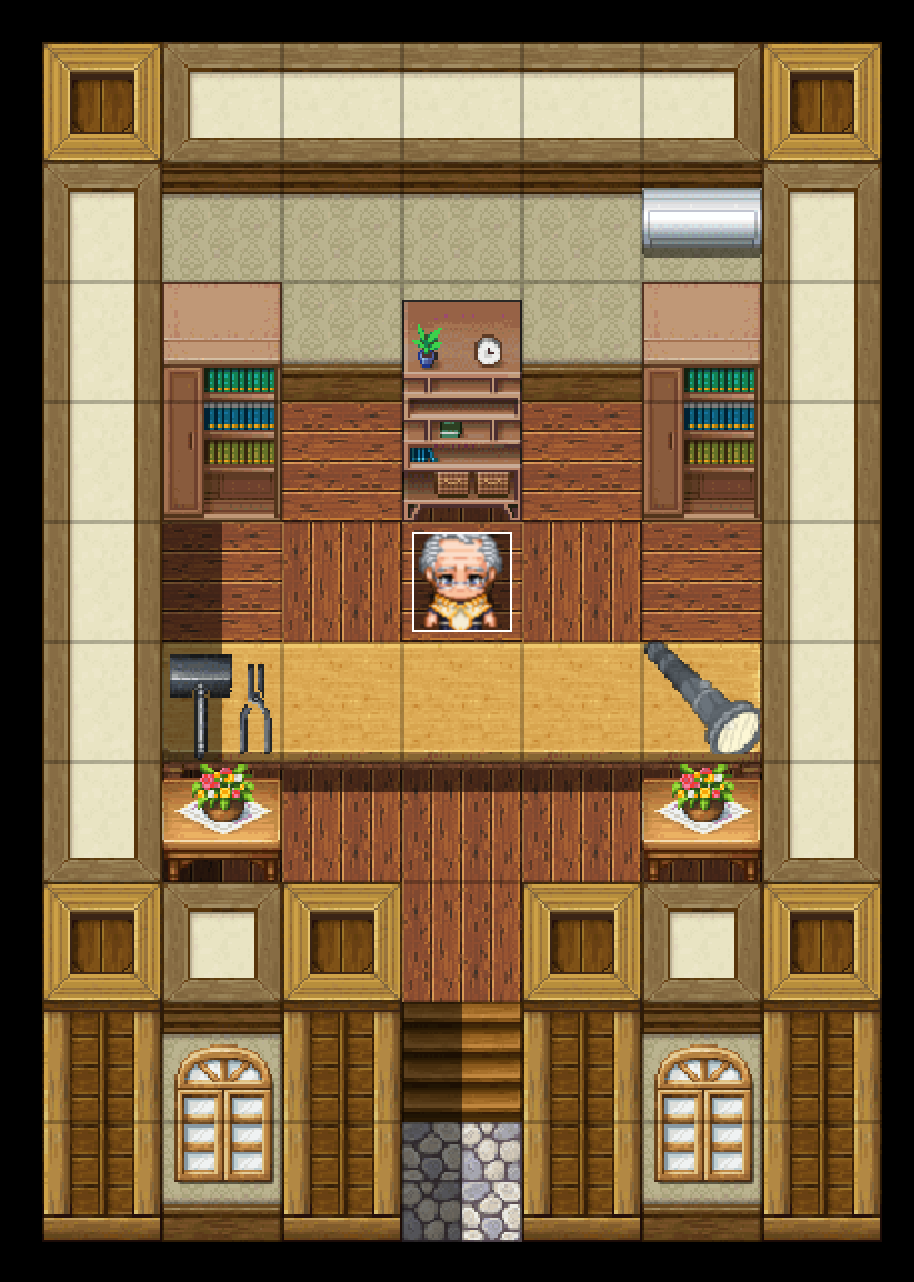
\includegraphics[scale=0.3]{Textuais/Pictures/Loja_Ferragens.png}
		      \fonte{Criado pelo autor.}\label{fig:loja-ferragens}
	      \end{figure}

	\item Casa do Chico: Espaço de união e diálogo da família, proporcionando um contraste com as áreas de mistério e aventura.

	      \begin{figure}[ht]
		      \centering
		      \caption{Mapa da casa do Chico.}
		      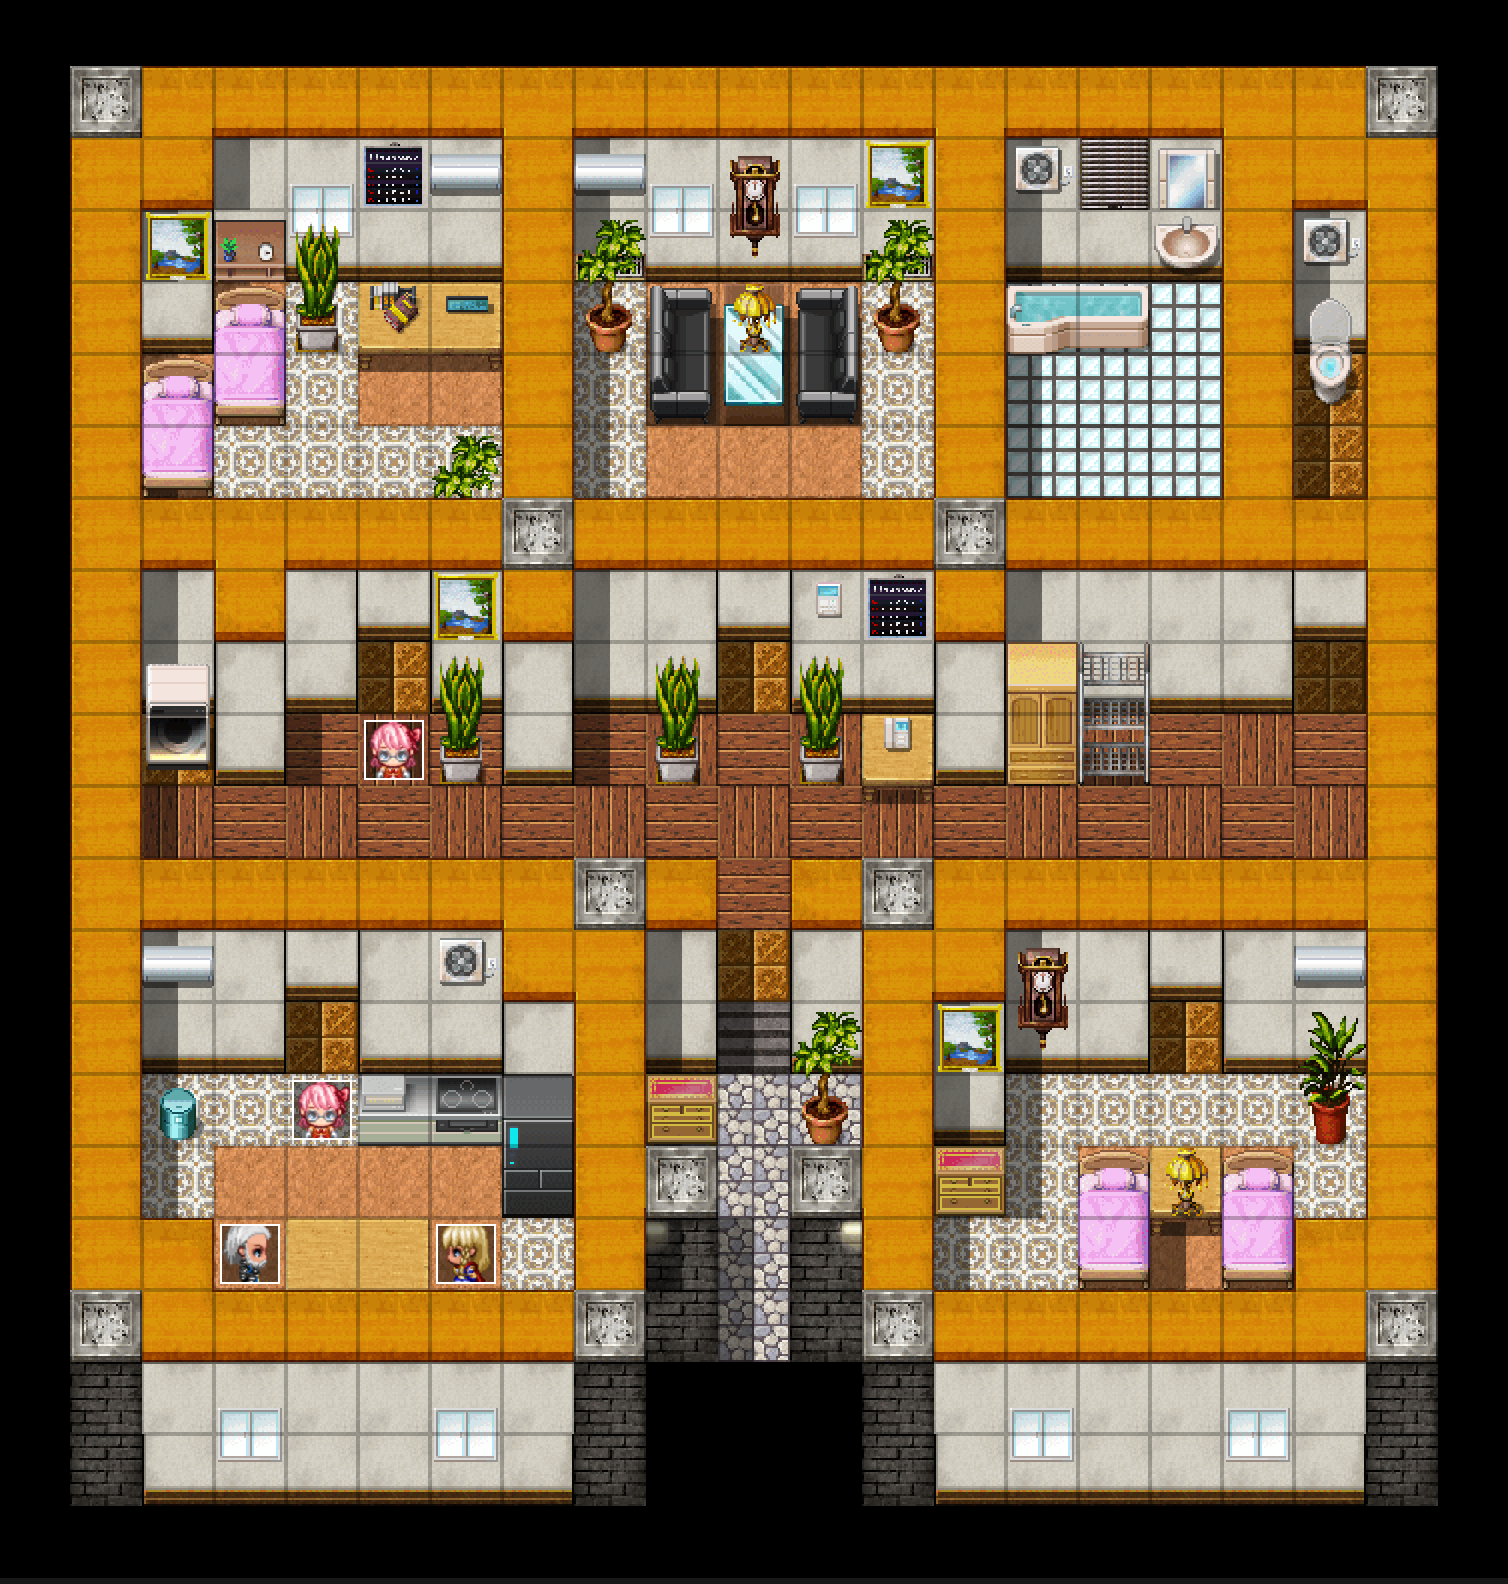
\includegraphics[scale=0.3]{Textuais/Pictures/Casa_chico.png}
		      \fonte{Criado pelo autor.}\label{fig:casa-chico}
	      \end{figure}
\end{itemize}
